\documentclass[10pt,a4paper]{article}
\usepackage[utf8]{inputenc}
\usepackage[T1]{fontenc}
\usepackage{graphicx}
\usepackage{float}
\usepackage{amsmath}
\usepackage{amsfonts}
\usepackage{amsthm}
\theoremstyle{definition}
\newtheorem{definition}{Definition}
\newtheorem{subdefinition}{Definition}[definition]
\theoremstyle{plain}
\newtheorem{example}{Example}[definition]

\title{Machine Learning 2023}
\author{David Graf}
\date{\today}
\begin{document}
	\maketitle
\part{Actual ML lecture content}
Recap of our setup:
\begin{enumerate}
	\item DOMAIN set X; we call $x\in X$ an instance
	\item LABEL set Y; e.g. $Y = \{0, 1\}$ (for a binary problem)
	\item TRAINING set $S = \big((x_1, y_1), ..., (x_m, y_m)\big)$  with $x_i \in X, y_i \in Y$
	\item a LEARNER that receives S and outputs 
	$$ h: X \to Y$$
	which we call a hypothesis
\end{enumerate}
Assumption: for now, we assume $x_i$'s are drawn iid from some probability measure D over the domain and labelled by some function (the labelling function) $f: X \to Y$:
$$ x_i \underbrace{ \sim }_{\text{\scriptsize"drawn from"}} D,\ y_i = f(x_i)$$

We are "interested" in 
$$D(\{x \in X: h(x) \neq f(x) \}) = \mathbb{P}_{X \sim D}[h(x) \neq f(x)] = L_{D, f}(h)$$
$L_{D, f}(h)$ is called the "Generalization Error" or "Risk".\\
The \underline{empirical version} of this is 
\begin{equation}
	\tag{[m] = \{1, ..., m\}}
	\frac{1}{m}\cdot\big|\big\{ i \in [m]: h(x_i) \neq f(x_i) \big\}\big| = L_S(h)
\end{equation}
the empirical error or empirical risk $L_S(h)$.
\paragraph{Convention:}
$S|_x = (x_1,..., x_m)$

\paragraph{Claim:}
ADD COMMENTS ON THE SIDE HERE, SLIDE 27
\begin{align*}
 \mathbb{E}_{S|_x \sim D^m}[L_S(H)] &= \mathbb{E}_{S|_x}\big[\frac{1}{m} \cdot \sum_{i=1}^{m} 1_{h(x_i) \neq f(x_i)}\big]\\
 &= \frac{1}{m} \cdot \sum_{i=1}^{m} \mathbb{E}_{x_i \sim D}[1_{h(x_i) \neq f(x_i)}] && \text{(by linearity of $\mathbb{E}$)}\\
 &= \frac{1}{m} \cdot \sum_{i=1}^{m} \mathbb{E}_{X \sim D}[1_{h(x) \neq f(x)}]\\
 &= \frac{1}{m} \cdot \sum_{i=1}^{m} \mathbb{P}_{X\sim D}[1_{h(x) \neq f(x)}]\\
 &=  \frac{1}{m} \cdot m \cdot \mathbb{P}_{X\sim D}[1_{h(x) \neq f(x)}]\\
 &= L_{D,f}(h)
\end{align*}

\paragraph{Our first learning paradigm} \underline{Empirical risk minimization (ERM)}:\\
As we only have access to the training data (S), it's natural to try to select \underline{h} such that the empirical risk is minimized. We call such an h an \underline{empirical risk minimizer} $(h_S)$.\\

\underline{A problematic case:}
\begin{figure}[H]
	\centering
	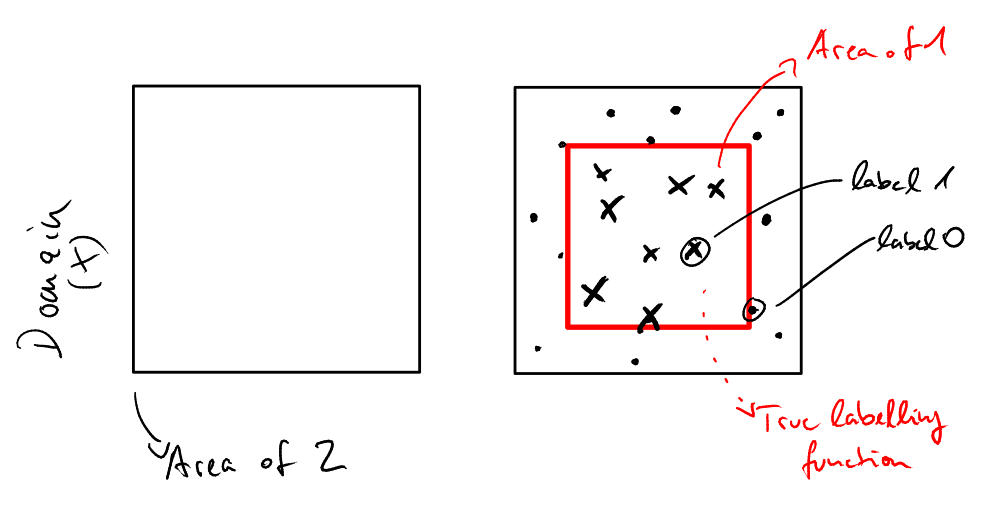
\includegraphics[width=0.7\linewidth]{sketch_1}
	\caption{Problematic Case 1}
	\label{fig:sketch1}
\end{figure}

\begin{itemize}
	\item say the distribution on X is uniform
	\item say we have an ERM algorithm that returns $h_S$ such that 
	\begin{align*}
			 h_s(x) &= \begin{cases}
			y_i , &  \text{if } \exists \ i \in [m]: x_i = x  \\
			0 , &  \text{else} 
		\end{cases} && \text{(a lookup table)} 
	\end{align*}
	Obviously $h_S$ is correct on our training set $$\implies L_S(h_S) = 0\text{ !}$$
	But on unseen instances from $D (X \sim D)$, $h_S$ is only correct 50\% of the time (due to the ratio of the areas of the black and red squares in the sketch): $$\implies L_{D,f}(h_S) = \frac{1}{2} \text{ !}$$
	This is called overfitting.
\end{itemize}

\paragraph{Hypothesis class (H):} We restrict searching for h to H, i.e., a class of functions from X to Y, and write:
$$
\text{ERM} = \text{ERM}_{H} (S) \in \text{argmin}_{h \in H} L_{S}(h)
$$
\underline{Remark:} In our previous example, we did not do this and allowed to memorize the training data!

\paragraph{ERM over finite hypothesis classes $(\big|H\big| < \infty)$:} 
$$\text{\underline{Assumption (realizability):} } \exists \ h^*\in H \text{ with } L_{D,f}(h^*) = 0$$
Now, any ERM hypothesis $h_S$ will attain 0 empirical error ($L_S(h_S) = 0$), as it computes with $h^*$ (which obviously has 0 empirical error).\\
\newline
Hence, $L_{D,f}(h_S) > \varepsilon$ can only happen if we select a hypothesis with $L_S(h_s) = 0$ but $L_{D,f}(h_S) > \varepsilon$ (trivially). We can write
\begin{align*}
	H_\text{BAD} = \{h \in H: L_{D,f}(h)>\varepsilon\} && \text{ set of BAD hypotheses}
\end{align*}
Also, we define
$$
	M = \{S|_x : \exists h \in \underbrace{H_{\text{BAD}}}_{\text{those are the ones with generalization error $> \varepsilon$}}, L_S(h) = 0  \}
$$

We observe
$$
\big\{S|_x : L_{D,f}(\underbrace{h_S}_{\text{ERM}}) \geq \varepsilon\big\} \subseteq  \underbrace{\big\{S|_x : \exists \ h \in H_{\text{BAD}}, L_S(h) = 0 \big\}}_{M = \cup_{h \in H_{\text{BAD}}}\{S|_x: L_{S}(h) = 0\} } = M
$$

We get (upon measuring with D):
\begin{align*}
D^m \big( \{S|_x : L_{D,f}(h_S) \geq \varepsilon\}\big) &\leq D^m\big( \cup_{h \in H_{\text{BAD}}}\{S|_x : L_{S}(h) = 0\} \big)\\
&\leq \sum_{h \in H_{\text{BAD}}} D^m \big(\{S|_x : L_{S}(h) = 0\}\big) && \text{(due to $\sigma$-sub-additivity)}
\end{align*}
\underline{Let's fix some $h \in H_{\text{BAD}}$:}
\begin{align*}
	D^m \big(\{S|_x : L_{S}(h) = 0\}\big) &= D^m \big(\{S|_x : \forall i \in [m]: h(x_i) = f(x_i)\}\big)\\
	&= \prod_{i = 1}^{n} D \big(\{x_i: h(x_i) = f(x_i)\}\big) && \text{(due to iid assumption)}\\
	&= \prod_{i=1}^{n} (1 - L_{D,f}(h))\\
	&\leq \prod_{i=1}^{n} (1-\varepsilon) && \text{(as $h \in H_{\text{BAD}}$)}\\
	&= (1-\varepsilon)^m \\
	&\leq e^{-\varepsilon m}
\end{align*}
So, to conclude:
\begin{align*}
	D^m \big(\{S|_x : L_{D,f}(h_S) \geq \varepsilon\}\big) &\leq \sum_{h \in H_{\text{BAD}}} e^{-\varepsilon m} \\ 
	&= |H_{\text{BAD}}| \cdot e^{-\varepsilon m} \\
	&\leq |H| \cdot e^{-\varepsilon m}
\end{align*}

\end{document}